\ifx\FORMAT\undefined
\documentclass[11pt]{book}
\usepackage{amsmath,mathtools}
\usepackage[utf8]{inputenc}
\usepackage[ngerman]{babel}
\usepackage{acronym}
\usepackage{graphicx} 
\usepackage{epstopdf}
\usepackage{svg}
\usepackage{multirow}
\usepackage{amssymb}
\usepackage{trfsigns}
\usepackage{setspace}
\usepackage{yfonts}
%\usepackage{HsKatitle11}

\onehalfspacing


%Hyperlinks package, links aus inhaltsverzeichnis
\usepackage{hyperref}
\hypersetup{
    colorlinks=false, %set true if you want colored links
    linktoc=all,
    linkbordercolor = {white}
}
%Blattformatierung
\usepackage{geometry}
\geometry{a4paper, top=25mm, left=30mm, right=25mm, bottom=20mm}

%Listing
\usepackage{courier}
\usepackage{listings}
\usepackage{color}
 \lstset{
   frame=tb,
   framexleftmargin=2.5em,
   basicstyle=\small\linespread{0.9}\bfseries\ttfamily,
   emph={square}, 
   emphstyle=\color{blue}\texttt,
   emph={[2]root,base},
   emphstyle={[2]\color{yac}\texttt},
   showstringspaces=false,
   flexiblecolumns=false,
   tabsize=2,
   numbers=left,
   numberstyle=\small\bfseries\ttfamily,
   numberblanklines=false,
   stepnumber=1,
   numbersep=10pt,
   xleftmargin=25pt
 }
 
 \def\presuper#1#2%
	{\mathop{}%
	\mathopen{\vphantom{#2}}^{#1}%
	\kern-\scriptspace%
	#2}
%Display vecotr in a reference frame
\newcommand{\vecBS}[4]{\presuper{#1}{\begin{pmatrix}
#2 \\ #3 \\ #4
\end{pmatrix}}}
%Boldsymbol shortcut
\newcommand{\bs}[1]{\boldsymbol{#1}}
%Bezugssystemdefinition
\newcommand{\defBS}[1]{\{#1\} [ \bs{e}_{{#1}_1},\bs{e}_{{#1}_2}, \bs{e}_{{#1}_3} ]}
%Projektionsmatrix
\newcommand{\pMat}[2]{\presuper{#1}{\bs{P}}^{#2}}
%Differenation in Respekt zu BS
\newcommand{\diffIn}[3]{\frac{\presuper{#1}{d{#2}}}{d#3}}
\newcommand{\partialDiffIn}[3]{\frac{\presuper{#1}{\partial{#2}}}{\partial #3}}
%Geschwindigkeit/Beschleunigung
\newcommand{\vel}[3]{\presuper{#1}{\bs{#2}}^{#3}}

%Rightarrow with spaceing
\newcommand{\rArrow}{\hspace{5pt}\rightarrow\hspace{5pt}}
%Inneres Produkt
\newcommand{\inProd}[2]{\langle {#1}, {#2} \rangle}

%System macro
\newcommand{\cSS}[3]{\textfrak{S}($\bs{#1}$,$\bs{#2}$,$\bs{#3}$)}
\newcommand{\dSS}[3]{\textfrak{D}($\bs{#1}$,$\bs{#2}$,$\bs{#3}$)}

%Laplace transform sign with spaces
\newcommand{\myLaplace}{\hspace{15pt}\laplace\hspace{15pt}}

\newcommand*{\signed}[1]{%
        \nolinebreak[3]\hspace*{\fill}\mbox{\emph{#1}}
    }
\begin{document}
\fi

\chapter{Modellbildung Würfel auf Ecke}\label{chapter_TM_Corner}
Das nächste Ziel besteht darin ein Regelungskonzept zu entwickeln, welches das Balancieren des Würfels auf einer Ecke ermöglicht. Hierfür werden drei Motor verwendet, wodurch das gesamte System über sechs Freiheitsgrade verfügt. Der erste Schritt besteht in dem Entwurf eines mechanischen Modells. Dieses führt zu einer Zustandsraumdarstellung, die als Grundlage für den Reglerentwurf verwendet wird.
Zu Beginn dieses Kapitels werden die Systemparameter vorgestellt, deren Bestimmung diskutiert und erste Annahmen getroffen um die weitere Modellbildung zu vereinfachen. Im zweiten Abschnitt wird die Kinematik des Systems untersucht. Hierbei werden zunächst die nötigen Bezugssysteme und generalisierten Koordinaten definiert, welche anschließend für die Bestimmung der generalisierten und partiellen Geschwindigkeiten benötigt werden.
Der nächste Abschnitt widmet sich der Kinematik. Hierunter fallen sowohl die wirkenden Drehmomente als auch die Trägheitsmomente der Körper. Daraus werden die generalisierten Kräfte und Trägheitskräfte ermittelt, welche nach Kanes Gleichungen auf die Bewegungsgleichungen führen. Diese werden anschließend in eine Zustandsraumdarstellung überführt.
\newpage
\section{Systemparameter}\label{TM_3D_Systemparameter}
Zunächst werden die Parameter des mechanischen Systems vorgestellt. Das System setzt sich aus drei Schwungmassen und dem Würfelkörper zusammen. Unter dem Würfelkörper ist das Würfelgehäuse inklusive der montierten Motoren, Sensoren und Elektrik zu verstehen und wird mit $K$ bezeichnet. Bei der Herleitung der Bewegungsgleichungen wird die Annahme getroffen, dass der Würfelkörper nicht translativ bewegt wird, sondern lediglich um Punkt $O$ rotiert. Der Punkt $O$ ist hierbei die Ecke auf welcher der Würfel balanciert. Des weiteren beschreiben alle Ortsvektoren den Vektor von $O$ zu dem jeweiligen Zielpunkt. Die drei Schwungmassen $R_i$ sind mit jeweils einem rotatorischem Freiheitsgrad auf den Motorwellen gelagert. Die Position der Lagerung wird mit $M_i$ bezeichnet und fällt auf Grund des symmetrischen Aufbau der Schwungmassen mit deren Schwerpunkt zusammen.
Die Massen
\begin{equation}
m_R = 0{,}155\text{ kg}
\end{equation}
und Trägheitstensoren $\bs{I}^{Ri/Mi}$ der Schwungmassen werden mit Hilfe der CAD-Anwendung ermittelt. 
Die Trägheitstensoren werden dabei aus der Perspektive des körperfesten Bezugssystem $K$ relativ zu den Punkten $M_i$ bestimmt. Für den Trägheitstensor der Schwungmasse $R_1$ ergibt sich der Wert
\begin{equation}
 \bs{I}^{R1/M1} = \begin{bmatrix}
3.358\cdot 10^{-4} & 2{,}641\cdot 10^{-11} & 0 
\\
2{,}651\cdot 10^{-11} & 1{,}961\cdot 10^{-4} & 4{,}527\cdot 10^{-9} 
\\
0 & 4.527\cdot 10^{-9} & 1{,}691\cdot 10^{-4}
\end{bmatrix} \text{ kg}\cdot \text{m}^2 \,.
\end{equation}
Hieran ist zu erkennen, dass die Vektorbasis des Bezugssystem $K$ nahezu den Haupträgheitsachsen der Schwungmasse entspricht, da die Devitationsmomente um die Größenordnung $10^{5}$ kleiner als die Haupträgheitsmomente sind. Deshalb wird bei der  
folgenden Untersuchung die Annahme getroffen, dass die Devitationsmomente vernachlässigt werden können und es gilt 
\begin{equation}
\begin{split}
\bs{I}^{R1/M1} &\equiv \begin{bmatrix}
I^{R1}_{11} & 0 & 0 \\ 0 & I^{R1}_{22} & 0 \\ 0 & 0 & I^{R1}_{33}
\end{bmatrix} = 
\begin{bmatrix}
3.358\cdot 10^{-4} & 0 & 0 \\
0 & 1{,}961\cdot 10^{-4} & 0 \\
0 & 0 & 1{,}691\cdot 10^{-4}
\end{bmatrix} \text{ kg}\cdot \text{m}^2
\\
\bs{I}^{R2/M2} &\equiv \begin{bmatrix}
I^{R2}_{11} & 0 & 0 \\ 0 & I^{R2}_{22} & 0 \\ 0 & 0 & I^{R2}_{33}
\end{bmatrix} = 
\begin{bmatrix}
1{,}691\cdot 10^{-4} & 0 & 0 \\
0 & 3.358\cdot 10^{-4} & 0 \\
0 & 0 & 1{,}961\cdot 10^{-4}
\end{bmatrix} \text{ kg}\cdot \text{m}^2
\\
\bs{I}^{R3/M3} &\equiv \begin{bmatrix}
I^{R3}_{11} & 0 & 0 \\ 0 & I^{R3}_{22} & 0 \\ 0 & 0 & I^{R3}_{33}
\end{bmatrix} = 
\begin{bmatrix}
1{,}961\cdot 10^{-4} & 0 & 0 \\
0 & 1{,}691\cdot 10^{-4} & 0 \\
0 & 0 & 3.358\cdot 10^{-4}
\end{bmatrix} \text{ kg}\cdot \text{m}^2 \,.
\end{split}
\end{equation}
Für die Masse des Würfelkörpers $m_K$ und des Gesamtsystems $m$ ergibt sich
\begin{equation}
m_K = 1{,}07 \text{ kg} \hspace{35pt} m = m_K + 3\cdot m_R = 1{,}532 \text{ kg}\,.
\end{equation}
Bei der Berechnung des Trägheittensors $\bs{I}^{GH/0}$ des Würfelkörpers um den Punkt $O$ wird der Einfluss der Schwungmassen nicht beachtet. Dies erfolgt bei der Berechnung der Trägheitsmomente in den folgenden Abschnitten. Somit ergibt sich für den Trägheitstensor
\begin{equation}
\begin{split}
\bs{I}^{GH/O} &= \begin{bmatrix}
I^{GH}_{11} & I^{GH}_{12} & I^{GH}_{13} \\
I^{GH}_{21} & I^{GH}_{22} & I^{GH}_{23} \\
I^{GH}_{31} & I^{GH}_{32} & I^{GH}_{33}
\end{bmatrix} \\
&=
\begin{bmatrix}
1{,}520\cdot 10^{-2} & -5{,}201\cdot 10^{-3} & 5{,}375\cdot 10^{-3} \\
-5{,}201\cdot 10^{-3} & 1{,}52\cdot 10^{-2} & 5{,}225\cdot 10^{-3} \\
5{,}375\cdot 10^{-3} & 5{,}225\cdot 10^{-3} & 1{,}542\cdot 10^{-2}
\end{bmatrix}\text{ kg}\cdot \text{m}^2 \,.
\end{split}
\end{equation}
Der Ortsvektor $\bs{c}$ des Schwerpunkt des Gesamtsystems wird ebenfalls numerisch ermittelt. Da sich die Komponenten des Ortsvektors $\bs{c}$ lediglich um $10^{-1}\text{mm}$ unterscheiden werden diese als identischen angenommen.
\begin{equation}
\bs{c} = \vecBS{K}{-6,61}{-6,60}{-6,57}\text{ cm} \approx \vecBS{K}{l_C}{l_C}{l_C} \hspace{15pt} \vert \hspace{15pt} l_C = 6,6\text{ cm}
\end{equation}
Des weiteren entsteht durch die Bewegung der Schwungmassen ein Reibmoment,welches als proportional zu den Winkelgeschwindigkeiten der Schwungmassen modelliert wird. Für Proportionalitätsfaktor $C_{\psi}$ wurde experimentell der  Wert 
\begin{equation}
C_{\psi} = 3,1176\cdot 10^{-5}\text{ kg}\cdot \text{m}^2 \cdot \text{s}^{-1}
\end{equation}
ermittelt.
\newpage
\section{Untersuchung der Kinematik}
Der erste Schritt in der Modellbildung besteht in der Definition der Bezugssysteme, welche zur Beschreibung der Systembewegung dienen. Der Ausgangspunkt ist das Inertialsystem $A$, welches durch die drei Einheitsvektoren $\bs{a}\idx1$, $\bs{a}\idx2$ und $\bs{a}\idx3$ definiert wird. Das Würfelgehäuse verfügt über drei rotatorische Freiheitsgrade, welche durch die Winkel $\varphi\idx1$, $\varphi\idx2$ und $\varphi\idx3$ beschrieben werden. 
\begin{figure}[!h]
\centering
\includegraphics[width=0.75\textwidth]{img/tm_corner_drawing.eps}
\caption{Mechanische Skizze des Würfels}
\end{figure}
Durch die Rotation des Würfels um den Winkel $\varphi\idx1$ in Richtung des Vektors $\bs{a}\idx1$ entsteht das Hilfsbezugssystem $B$, welches durch die Einheitsvektoren $\bs{b}\idx1$, $\bs{b}\idx2$ und $\bs{b}\idx3$ definiert wird. Für die Abbildungsmatrix gilt
\begin{equation}
\pMat{A}{B} = \begin{bmatrix}
1 & 0 & 0 \\ 0 & c_{\varphi\idx1} & s_{\varphi\idx1} \\ 0 & -s_{\varphi\idx1} & c_{\varphi\idx1}
\end{bmatrix} \,.
\end{equation}
Die Rotation um den Winkel $\varphi\idx2$ in Richtung des Vektors $\bs{b}\idx2$ führt zu dem zweiten Hilfsbezugssystem $C$ mit den drei Einheitsvektoren $\bs{c}\idx1$, $\bs{c}\idx2$ und $\bs{c}\idx3$ und der Projektionsmatrix
\begin{equation}
\pMat{B}{C} = \begin{bmatrix}
c_{\varphi\idx2} & 0 & -s_{\varphi\idx2} \\
0 & 1 & 0 \\
 s_{\varphi\idx2} & 0 & c_{\varphi\idx2}
\end{bmatrix} \,.
\end{equation}
Die letzte Rotation des Würfels in Richtung von $\bs{c}\idx3$ um den Winkel $\varphi\idx3$ führt zu dem körperfesten Bezugssystem $K$, welches durch die drei Vektoren $\bs{k}\idx1$, $\bs{k}\idx2$ und $\bs{k}\idx3$ definiert ist. Für die Abbildungsmatrix gilt 
\begin{equation}
\pMat{C}{K} = \begin{bmatrix}
c_{\varphi\idx3} & s_{\varphi\idx3} & 0 \\ -s_{\varphi\idx3} & c_{\varphi\idx3} & 0 \\ 0 & 0 & 1
\end{bmatrix} \,.
\end{equation}
Hier sei angemerkt, dass es sich bei den Bezugssystemen $B$ und $C$ um theoretische Konstrukte handelt, für die kein physisches Gegenstück existiert. Sie werden lediglich als Hilfsmittel zur Beschreibung des Systems verwendet (\cite{KaneBook}, S. 24 ff.).

Durch die Rotation der Schwungmassen besitzt das System drei weitere Freiheitsgrade, welche von den Winkeln $\psi\idx1$, $\psi\idx2$ und $\psi\idx3$ beschrieben werden. Somit entstehen drei weitere Bezugssysteme, deren Vektorbasen jeweils an den Schwungmassen fixiert sind. Allerdings spielen diese keine weitere Rolle, da es sich bei den Winkeln $\psi_i$ um zyklische Koordinaten handelt. Das heißt, dass der Impuls des Systems nicht von der Ausrichtung der Schwungmassen beeinflusst wird. Lediglich die Winkelgeschwindigkeiten $\dot{\psi}_i$ wirken auf Grund der Reibung auf das System.

Die Position und Ausrichtung des Systems wird von den sechs Winkeln $\varphi_i$ und $\psi_i$ vollständig beschrieben. Deshalb werden diese als generalisierte Koordinaten 
\begin{equation}
q_i \equiv \varphi_i \hspace{35pt} q_j \equiv \psi_i \hspace{35pt} (i=1,2,3, j=4,5,6) \,.
\end{equation}
Mit Hilfe der Bezugssysteme und generalisierten Koordinaten können nun die Winkelgeschwindigkeit des Würfels $\vel{A}{\omega}{K}$ und der Schwungmassen $\vel{A}{\omega}{R_i}$ bestimmt werden. Diese ergeben sich aus der Addition der relativen Rotationsgeschwindigkeiten der Bezugssysteme zueinander (\cite{KaneBook}, S. 24).
\begin{equation}
\begin{split}
\vel{A}{\omega}{K} &= \vel{A}{\omega}{B}+\vel{B}{\omega}{C}+\vel{C}{\omega}{K} = \vecBS{A}{\dot{\varphi}\idx1}{0}{0} + \vecBS{B}{0}{\dot{\varphi}\idx2}{0} + \vecBS{C}{0}{0}{\dot{\varphi}\idx3} \\
&= \vecBS{K}
{\dot{\varphi}\idx2\cdot s_{\varphi\idx3} + \dot{\varphi}\idx1 \cdot c_{\varphi\idx2}\cdot c_{\varphi\idx3}}
{\dot{\varphi}\idx2\cdot c_{\varphi\idx3} - \dot{\varphi}\idx1 \cdot c_{\varphi\idx2}\cdot s_{\varphi\idx3}}
{\dot{\varphi}\idx3 + \dot{\varphi}\idx1\cdot s_{\varphi\idx2}}
\end{split}
\end{equation}
Die Winkelgeschwindigkeiten der Schwungmassen $\vel{K}{\omega}{R_i}$ relativ zu dem Würfel entsprechen der ersten Ableitung der Winkel $\psi_i$. Mit Hilfe des Additionstheorems für Winkelgeschwindigkeiten kann daraus auch die absolute Winkelgeschwindigkeit der Schwungmassen 
\begin{equation}
\vel{K}{\omega}{R_1} = \vecBS{K}{\dot{\psi}\idx1}{0}{0} \hspace{35pt}
\vel{K}{\omega}{R_2} = \vecBS{K}{0}{\dot{\psi}\idx2}{0} \hspace{35pt}
\vel{K}{\omega}{R_3} = \vecBS{K}{0}{0}{\dot{\psi}\idx3} 
\end{equation}
\begin{equation}
\vel{A}{\omega}{R_i} = \vel{A}{\omega}{K} + \vel{K}{\omega}{R_i} \hspace{35pt} (i=1,2,3)
\end{equation}
berechnet werden. Im nächsten Schritt werden die absoluten Geschwindigkeiten der Teilsysteme in Komponenten zerlegt, welche sich aus den generalisierten Geschwindigkeiten $u_i$ und partiellen Geschwindigkeiten $\vel{A}{\omega}{j}_i$ zusammensetzen. Hierfür müssen zu nächst die generalisierten Geschwindigkeiten $u_i$ definiert werden. An dieser Stelle sei erwähnt, dass die Definition der generalisierten Geschwindigkeiten die Form der resultierenden Bewegungsgleichungen stark beeinflusst. Das letztendliche Ziel bei der Wahl der generalisierten Geschwindigkeiten ist es möglichst einfache Bewegungsgleichungen zu erhalten. Dies wird erreicht , in dem die generalisierten Geschwindigkeiten so gewählt werden, dass die Geschwindigkeiten der Körper im Intertialsystem auf möglichst einfache Terme reduziert werden (\cite{KanePaper}). Nach diesem Ansatz werden die  generalisierten Geschwindigkeiten 
\begin{equation}
\begin{split}
u\idx1 &= \dot{\varphi}\idx2\cdot s_{\varphi\idx3} + \dot{\varphi}\idx1\cdot c_{\varphi\idx2}\cdot c_{\varphi\idx3} \\
u\idx2 &= \dot{\varphi}\idx2\cdot c_{\varphi\idx3} - \dot{\varphi}\idx1\cdot c_{\varphi\idx2}\cdot s_{\varphi\idx3} \\
u\idx3 &= \dot{\varphi}\idx3 + \dot{\varphi}\idx1\cdot s_{\varphi\idx2} \\
u_4 &= \dot{\varphi}\idx2\cdot s_{\varphi\idx3} + \dot{\varphi}\idx1\cdot c_{\varphi\idx2}\cdot c_{\varphi\idx3} + \dot{\psi}\idx1 \\
u_5 &= \dot{\varphi}\idx2\cdot c_{\varphi\idx3} - \dot{\varphi}\idx1\cdot c_{\varphi\idx2}\cdot s_{\varphi\idx3} + \dot{\psi}\idx2 \\
u_6 &= \dot{\varphi}\idx3 + \dot{\varphi}\idx1\cdot s_{\varphi\idx2} + \dot{\psi}\idx3
\end{split}
\end{equation}
gewählt. Mit diesen Definitionen können die Winkelgeschwindigkeiten der Körper im A in die Form 
\begin{equation}
\vel{A}{\omega}{K} = \vecBS{K}{u\idx1}{u\idx2}{u\idx3}, \vel{A}{\omega}{R1} = \vecBS{K}{u\idx4}{u\idx2}{u\idx3}, \vel{A}{\omega}{R2} = \vecBS{K}{u\idx1}{u\idx5}{u\idx3}, \vel{A}{\omega}{R3} = \vecBS{K}{u\idx1}{u\idx2}{u\idx6}
\end{equation}
gebracht werden. Die Einführung der generalisierten Geschwindigkeiten führt einerseits zu einem einfachen  Ausdruck der absoluten Winkelgeschwindigkeiten aus Perspektive des körperfesten Bezugssystem $K$. Andererseits können dadurch auch die partiellen Geschwindigkeiten $\vel{A}{\omega}{j}_i$ in einfachen Termen ausgedrückt werden. Für diese gilt 
\begin{align}
\vel{A}{\omega}{K} &= u\idx1 \cdot \bs{k}\idx1 + u\idx2 \cdot \bs{k}\idx2 + u\idx3 \cdot \bs{k}\idx3 &\rArrow &\vel{A}{\omega}{K}\idx1 = \bs{k}\idx1, \vel{A}{\omega}{K}\idx2 = \bs{k}\idx2, \vel{A}{\omega}{K}\idx3 = \bs{k}\idx3 \\
& & &\vel{A}{\omega}{K}\idx4 = 0, \vel{A}{\omega}{K}\idx5 = 0, \vel{A}{\omega}{K}\idx6 = 0 \nonumber
\\
\vel{A}{\omega}{R\idx1} &= u\idx4 \cdot \bs{k}\idx1 + u\idx2 \cdot \bs{k}\idx2 + u\idx3 \cdot \bs{k}\idx3 &\rArrow 
&\vel{A}{\omega}{K}\idx1 = 0, \vel{A}{\omega}{K}\idx2 = \bs{k}\idx2, \vel{A}{\omega}{K}\idx3 = \bs{k}\idx3 \\
& & &\vel{A}{\omega}{K}\idx4 = \bs{k}\idx1, \vel{A}{\omega}{K}\idx5 = 0, \vel{A}{\omega}{K}\idx6 = 0 \nonumber
\\
\vel{A}{\omega}{R\idx2} &= u\idx1 \cdot \bs{k}\idx1 + u\idx5 \cdot \bs{k}\idx2 + u\idx3 \cdot \bs{k}\idx3&\rArrow 
&\vel{A}{\omega}{K}\idx1 = \bs{k}\idx1, \vel{A}{\omega}{K}\idx2 = 0, \vel{A}{\omega}{K}\idx3 = \bs{k}\idx3 \\
& & &\vel{A}{\omega}{K}\idx4 = 0, \vel{A}{\omega}{K}\idx5 = \bs{k}\idx2, \vel{A}{\omega}{K}\idx6 = 0 \nonumber
\\
\vel{A}{\omega}{R\idx3} &= u\idx1 \cdot \bs{k}\idx1 + u\idx2 \cdot \bs{k}\idx2 + u\idx6 \cdot \bs{k}\idx3&\rArrow 
&\vel{A}{\omega}{K}\idx1 = \bs{k}\idx1, \vel{A}{\omega}{K}\idx2 = \bs{k}\idx2, \vel{A}{\omega}{K}\idx3 = 0 \\
& & &\vel{A}{\omega}{K}\idx4 = 0, \vel{A}{\omega}{K}\idx5 = 0, \vel{A}{\omega}{K}\idx6 = \bs{k}\idx3 \nonumber \,
\end{align}
Die Beudeutung der generalisierten und partiellen Geschwindigkeiten kann so interpretiert werden, dass sie eine Unterteilung der Bewegung in Betrag und Richtung darstellen. Die generalisierten Geschwindigkeiten geben als skalare Größen den Betrag der Geschwindigkeit wieder, wobei die entsprechenden partiellen Geschwindigkeiten die Bewegungsrichtung darstellen.

\newpage
\section{Untersuchung der Kinetik}
Der nächste Schritt besteht darin die Kräfte zu modellieren, welche auf den Würfelkörper und die drei Schwungmassen wirken. Aus diesen können im Anschluss mit Hilfe der partiellen Geschwindigkeiten die generalisierten aktiven Kräfte $F_i$ ermittelt werden.
Zunächst sollen die resultierenden Drehmomente $\bs{T}^{Ri/Mi}$ der Schwungmassen $R_i$ um ihren jeweiligen Drehpunkt $M_i$ bestimmt werden. Hierfür muss einerseits das Drehmoment $\bs{T}^{Ri/Mi}_M$ des antreibenden Motors und das verzögernde Reibmoment $\bs{T}^{Ri/Mi}_R$ beachtet werden.
Diese ergeben sich aus der Summe der Drehmomente $\bs{T}^{Ri/Mi}$, welche durch die antreibenden Motoren verursacht werden, und der verzögernden Reibmomente $\bs{T}^{Ri/Mi}$
\begin{equation}
\bs{T}^{R1/M1} = \bs{T}^{R1/M1}_M + \bs{T}^{R1/M1}_R = \vecBS{K}{T_{M1}}{0}{0} + \vecBS{K}{-C_{\psi}\cdot (u_4 - u_1)}{0}{0}
\end{equation}
\begin{equation}
\bs{T}^{R2/M2} = \bs{T}^{R2/M2}_M + \bs{T}^{R2/M2}_R = \vecBS{K}{0}{T_{M2}}{0} + \vecBS{K}{0}{-C_{\psi}\cdot (u_5 - u_2)}{0}
\end{equation}
\begin{equation}
\bs{T}^{R3/M3} = \bs{T}^{R3/M3}_M + \bs{T}^{R3/M3}_R = \vecBS{K}{0}{0}{T_{M3}} + \vecBS{K}{0}{0}{-C_{\psi}\cdot (u_6 - u_3)}\,.
\end{equation}
Der Würfelkörper wird einerseits durch das Gravitationsmoment $\bs{T}^{K/O}_G$ und die resultierenden Momente der Schwungmassen $\bs{T}^{Ri/Mi}$, welche in umgekehrter Richtung auf den Würfel wirken, beeinflusst.
Das Gravitationsmoment hängt von der Gewichtskraft $\bs{G}$ und der Position des Schwerpunktes $\bs{c}$ ab.
\begin{equation}
\begin{split}
\bs{T}^{K/O}_G &= \bs{c} \times \bs{G} = \vecBS{K}{l_C}{l_C}{l_C} \times \vecBS{K}{-m\cdot g \cdot c_{\varphi_2} \cdot c_{\varphi_3}}{-m\cdot g\cdot c_{\varphi_2}\cdot s_{\varphi_3}}{-m\cdot g\cdot s_{\varphi_2}} 
\\
&= -m\cdot l_C \cdot g \vecBS{K}{s_{\varphi_2}+c_{\varphi_2}s_{\varphi_3}}
{-s_{\varphi_2}+c_{\varphi_2}c_{\varphi_3}}
{-c_{\varphi_2}c_{\varphi_3} - c_{\varphi_2}\cdot s_{\varphi_3}}
\end{split}
\end{equation}
Somit folgt für das resultierende Drehmoment
\begin{equation}
\begin{split}
\bs{T}^{K/O}&=\bs{T}^{K/O}_G - \bs{T}^{R1/M1} - \bs{T}^{R2/M2} - \bs{T}^{R3/M3} \\
&= -m\cdot l_C \cdot g \vecBS{K}{s_{\varphi_2}+c_{\varphi_2}s_{\varphi_3}}
{-s_{\varphi_2}+c_{\varphi_2}c_{\varphi_3}}
{-c_{\varphi_2}c_{\varphi_3} - c_{\varphi_2}\cdot s_{\varphi_3}} - \vecBS{K}{T_{M1}-C_{\psi}(u_4 - u_1)}{T_{M2}-C_{\psi}(u_5 - u_2)}{T_{M3}-C_{\psi}(u_6 - u_3)}
\end{split}\,.
\end{equation}
Im nächsten Schritt können die generalisierten aktiven Kräfte berechnet werden. Diese entsprechen der Summe der inneren Produkte der resultierenden Drehmomente und der  partiellen Geschwindigkeit der Körper. Wenn die partiellen Geschwindigkeiten als die  Bewegungsrichtungen der Körper betrachtet werden, so stellt die Skalarmultiplikation der partiellen Geschwindigkeit und dem resultierenden Drehmoments dessen Abbildung in die Bewegungsrichtung dar. Folglich handelt es sich bei den generalisierten aktiven Kräften um skalare Größen, welche den Einfluss der wirkenden Drehmomente in Richtung der Freiheitsgrade wiedergeben.
\begin{align}
F_1 &= \inProd{\vel{A}{\omega}{K}_1}{\bs{T}^{K/O}} + \sum^3_{i=1} \inProd{\vel{A}{\omega}{Ri}_1}{\bs{T}^{Ri/Mi}} 
\\
&= m\cdot l_C \cdot g (-s_{\varphi_2}-c_{\varphi_2}s_{\varphi_3}) - T_{M1} + C_{\psi}(u_4 - u_1) \nonumber
\\
F_2 &= \inProd{\vel{A}{\omega}{K}_2}{\bs{T}^{K/O}} + \sum^3_{i=1} \inProd{\vel{A}{\omega}{Ri}_2}{\bs{T}^{Ri/Mi}} 
\\
&= m\cdot l_C \cdot g (s_{\varphi_2}-c_{\varphi_2}c_{\varphi_3})-T_{M2}+C_{\psi}(u_5 - u_2) \nonumber
\\
F_3 &= \inProd{\vel{A}{\omega}{K}_3}{\bs{T}^{K/O}} + \sum^3_{i=1} \inProd{\vel{A}{\omega}{Ri}_3}{\bs{T}^{Ri/Mi}} 
\\
&= m\cdot l_C \cdot g (c_{\varphi_2}c_{\varphi_3} + c_{\varphi_2}s_{\varphi_3}) - T_{M3} + C_{\psi}(u_6 - u_3) \nonumber
\\
F_4 &= \inProd{\vel{A}{\omega}{K}_4}{\bs{T}^{K/O}} + \sum^3_{i=1} \inProd{\vel{A}{\omega}{Ri}_4}{\bs{T}^{Ri/Mi}} = T_{M1}-C_{\psi}(u_4 - u_1)
\\
F_5 &= \inProd{\vel{A}{\omega}{K}_5}{\bs{T}^{K/O}} + \sum^3_{i=1} \inProd{\vel{A}{\omega}{Ri}_5}{\bs{T}^{Ri/Mi}} = T_{M2}-C_{\psi}(u_5 - u_2)
\\
F_6 &= \inProd{\vel{A}{\omega}{K}_6}{\bs{T}^{K/O}} + \sum^3_{i=1} \inProd{\vel{A}{\omega}{Ri}_6}{\bs{T}^{Ri/Mi}} = T_{M3}-C_{\psi}(u_6 - u_3)
\end{align}
Neben den aktiven Kräften müssen auch die generalisierten Trägheitskräfte $F^*_i$ ermittelt werden um die Bewegungsgleichungen zu bestimmen. Hierfür werden zunächst die Trägheitsmomente $\bs{T}_*$ der Körper ermittelt werden. Nach (\cite{KaneBook}, S. 124 ff.) gilt für die Trägheitsmomente der  Zusammenhang
\begin{equation}
\bs{T}_* = -\bs{\alpha}\cdot \bs{I} - \bs{\omega}\times(\bs{I}\cdot\bs{\omega}) \,.
\end{equation}
Wobei $\bs{\alpha}$ und $\bs{\omega}$ die Winkelbeschleunigung bzw. -geschwindigkeit des Körpers und $\bs{I}$ dessen Trägheitstensor bezeichnet. 
Die Winkelgeschwindigkeiten der Körper sind bereits bekannt, die Winkelbeschleunigung ergeben sich durch die Ableitung der Winkelgeschwindigkeiten relativ zu dem Intertialsystem $A$.
\begin{equation}
\vel{A}{\alpha}{K} = \frac{\presuper{A}d}{dt}\vel{A}{\omega}{K}, \vel{A}{\alpha}{R1} = \frac{\presuper{A}d}{dt}\vel{A}{\omega}{R1}, \vel{A}{\alpha}{R2} = \frac{\presuper{A}d}{dt}\vel{A}{\omega}{R2}, \vel{A}{\alpha}{R3} = \frac{\presuper{A}d}{dt}\vel{A}{\omega}{R3}
\end{equation}
Zunächst sollen die Trägheitsmomente $\bs{T}^{Ri/Mi}_*$ der Schwungmassen bestimmt werden. Deren Trägsheitstensoren $\bs{I}^{Ri/Mi}$ im Bezug auf die Drehpunkte $M_i$ wurde, wie in Abschnitt (\ref{TM_3D_Systemparameter}) erläutert, mit Hilfe einer CAD-Anwendung ermittelt.
\begin{equation}
\bs{I}^{Ri/Mi} = \begin{pmatrix}
I^{Ri}_{11} & 0 & 0 \\ 0 & I^{Ri}_{22} & 0 \\ 0 & 0 & I^{Ri}_{33}
\end{pmatrix}
\end{equation}
\begin{equation}
\bs{T}^{Ri/Mi}_* = - \vel{A}{\alpha}{Ri} - \vel{A}{\omega}{Ri}\times(\bs{I}^{Ri/Mi} \cdot \vel{A}{\omega}{Ri})
\end{equation}
Der Trägheitstensor $\bs{I}^{K/O}$ des Würfelkörpers um den Punkt $O$ setzt sich aus mehreren Komponenten zusammen. Einerseits wird er durch den Trägheitstensor $\bs{I}^{GH/O}$ des Gehäuses um den Punkt $O$ beeinflusst, dieser Tensor beschreibt die Trägheitseigenschaften des Würfels ohne die Schwungmassen zu berücksichtigen. Andererseits beeinflussen die Schwungmassen das Trägheitsmoment des Würfelkörpers. Um diesen Einfluss nachzuvollziehen wird die Bewegung der Schwungmassen in zwei Komponenten zerlegt. Einerseits rotieren die Schwungmassen $R_i$ um die Punkte $M_i$, welche die Schwerpunkte der Schwungmassen sind. Andererseits bewegen sich die Schwerpunkte $M_i$ um den Punkt $O$ und sind bei der Betrachtung der Trägheitseigenschaften dem Würfelkörper zuzuordnen. Der Grund hierfür ist, dass die Schwerpunkte der Schwungmassen auf dem Würfelkörper fixiert sind. Im Modell werden die Schwerpunkte als Punktmassen mit der Masse $m_R$ behandelt. Diese Interpretation entspricht der Aussage des Steiner'schen Satzes.
Somit ist der Trägheitstensor $\bs{I}^{K/O}$ gleich der Summe von $\bs{I}^{GH/O}$ und den Trägheitstensoren der drei Massepunkte $M_i$ mit der Masse $m_R$ um $O$, wobei $\bs{r}_i$ den Ortsvektor des Punktes $M_i$ beschreibt.
\begin{equation}
\bs{I}^{K/O} = \bs{I}^{GH/O} + \sum^3_{i=1}m_R(\inProd{\bs{r}_i}{\bs{r}_i}-\bs{r}_i\otimes\bs{r}_i)
\end{equation}
\begin{equation}
\bs{T}^{K/O}_* = - \vel{A}{\alpha}{K}\cdot\bs{I}^{K/O} - \vel{A}{\omega}{K}\times(\bs{I}^{K/O}\cdot \vel{A}{\omega}{K})
\end{equation}
Prinzipiell können nun die generalisierten Trägheitskräfte $F^*_i$ durch die Skalarmultiplikation mit den partiellen Geschwindigkeiten berechnet werden. Allerdings handelt es sich bei den Trägheitsmomenten um nichtlineare Terme. Diese führen einerseits auf schwer nachzuvollziehende Bewegungsgleichungen. Andererseits werden für die Transformation in eine Zustandsraumdarstellung lineare Differentialgleichungen benötigt. In diesem Fall kann eine vorzeitige Linearisierung durchgeführt werden (\cite{KaneBook}, S. 171 ff.). Das heißt an Stelle die vollständigen, nicht linearen Bewegungsgleichungen zu bestimmen und anschließend zu linearisieren, werden bereits die generalisierten  Geschwindigkeiten $\hat{\bs{\omega}}$, sowie die resultierenden Dreh- und Trägheitsmomente $\hat{F}_i$ und $\hat{F}^*_i$ linearisiert und daraus die linearen Bewegungsgleichungen bestimmt.
Hierfür muss zunächst der Arbeitspunkt des Systems festgelegt werden, welcher der Position auf eine rEcke entspricht. Die Winkel $\varphi_i$ müssen folglich so gewählt werden, dass der Ortsvektor des Schwerpunktes $\bs{c}$ aus Perspektive des Inertialsystems lediglich eine Komponente in Richtung von $\bs{a}_1$ besitzt.
\begin{equation}
\vecBS{A}{\vert \bs{c} \vert}{0}{0} \overset{!}= \pMat{K}{A}\cdot \vecBS{K}{l_C}{l_C}{l_C} \rArrow \varphi_{10} = 0, \hspace{10pt} \varphi_{20} =-2\cdot \text{atan}(\sqrt{2}-\sqrt{3}), \hspace{10pt} \varphi_{30}=\frac{-\pi}{4}
\end{equation}
\begin{equation}
\hat{\varphi}_i = \varphi_{i0} + \bar{\varphi}_i
\end{equation}
In dem Gleichgewichtspunkt verschwinden die Winkelgeschwindigkeiten des Systems, folglich gilt für die generalisierten Geschwindigkeiten im Arbeitspunkt $u_{i0} = 0$
\begin{align}
\hat{u}_1 &= \dot{\varphi}_2\cdot s_{\varphi_{30}} + \dot{\varphi}_1\cdot c_{\varphi_{20}}c_{\varphi_{30}} \\
\hat{u}_2 &= \dot{\varphi}_2\cdot c_{\varphi_{30}} - \dot{\varphi}_1\cdot c_{\varphi_{20}} s_{\varphi_{30}} \\
\hat{u}_3 &= \dot{\varphi}_3 + \dot{\varphi}_1\cdot s_{\varphi_{20}} \\
\hat{u}_4 &= \dot{\varphi}_2\cdot s_{\varphi_{30}} + \dot{\varphi}_1\cdot c_{\varphi_{20}} c_{\varphi_{30}} + \dot{\psi}_1 \\
\hat{u}_5 &= \dot{\varphi}_2\cdot c_{\varphi_{30}} - \dot{\varphi}_1\cdot c_{\varphi_{20}}s_{\varphi_{30}} + \dot{\psi}_2 \\
\hat{u}_6 &= \dot{\varphi}_3 + \dot{\varphi}_1\cdot s_{\varphi_{20}} + \dot{\psi}_3
\end{align}
\begin{equation}
\vel{A}{\hat{\omega}}{K} = \vecBS{K}{\hat{u}_1}{\hat{u}_2}{\hat{u}_3}, \hspace{10pt} \vel{A}{\hat{\omega}}{R1} = \vecBS{K}{\hat{u}_4}{\hat{u}_2}{\hat{u}_3}, \hspace{10pt}
\vel{A}{\hat{\omega}}{R2} = \vecBS{K}{\hat{u}_1}{\hat{u}_5}{\hat{u}_3}, \hspace{10pt}
\vel{A}{\hat{\omega}}{R3} = \vecBS{K}{\hat{u}_1}{\hat{u}_2}{\hat{u}_6} \,.
\end{equation}
Insbesondere die Winkelbeschleunigungen werden durch die linearisierten Winkelgeschwindigkeiten stark vereinfacht.
\begin{align}
\vel{A}{\hat{\alpha}}{K} &= {\presuper{A}d}{dt}\vel{A}{\hat{\omega}}{K}
 &&= \vecBS{K}{\ddot{\varphi}_2\cdot s_{\varphi_{30}} + \ddot{\varphi}_1\cdot c_{\varphi_{20}}c_{\varphi_{30}}}{\ddot{\varphi}_2\cdot c_{\varphi_{30}} - \ddot{\varphi}_1\cdot c_{\varphi_{20}} s_{\varphi_{30}}}{\ddot{\varphi}_3 + \ddot{\varphi}_1\cdot s_{\varphi_{20}}} &&= \vecBS{K}{\hat{\dot{u}}_1}{\hat{\dot{u}}_2}{\hat{\dot{u}}_3}
\\
\vel{A}{\hat{\alpha}}{R1} &= \frac{\presuper{A}d}{dt}\vel{A}{\hat{\omega}}{R1} &&= \vecBS{K}{\ddot{\varphi}_2\cdot s_{\varphi_{30}} + \ddot{\varphi}_1\cdot c_{\varphi_{20}}c_{\varphi_{30}}+\ddot{\psi}_1}{\ddot{\varphi}_2\cdot c_{\varphi_{30}} - \ddot{\varphi}_1\cdot c_{\varphi_{20}} s_{\varphi_{30}}}{\ddot{\varphi}_3 + \ddot{\varphi}_1\cdot s_{\varphi_{20}}} &&= \vecBS{K}{\hat{\dot{u}}_4}{\hat{\dot{u}}_2}{\hat{\dot{u}}_3}
\\
\vel{A}{\hat{\alpha}}{R2} &= \frac{\presuper{A}d}{dt}\vel{A}{\hat{\omega}}{R2} &&= \vecBS{K}{\ddot{\varphi}_2\cdot s_{\varphi_{30}} + \ddot{\varphi}_1\cdot c_{\varphi_{20}}c_{\varphi_{30}}}{\ddot{\varphi}_2\cdot c_{\varphi_{30}} - \ddot{\varphi}_1\cdot c_{\varphi_{20}} s_{\varphi_{30}} + \ddot{\psi}_2}{\ddot{\varphi}_3 + \ddot{\varphi}_1\cdot s_{\varphi_{20}}} &&= \vecBS{K}{\hat{\dot{u}}_1}{\hat{\dot{u}}_5}{\hat{\dot{u}}_3}
\\
\vel{A}{\hat{\alpha}}{K} &= \frac{\presuper{A}d}{dt}\vel{A}{\hat{\omega}}{K} &&= \vecBS{K}{\ddot{\varphi}_2\cdot s_{\varphi_{30}} + \ddot{\varphi}_1\cdot c_{\varphi_{20}}c_{\varphi_{30}}}{\ddot{\varphi}_2\cdot c_{\varphi_{30}} - \ddot{\varphi}_1\cdot c_{\varphi_{20}} s_{\varphi_{30}}}{\ddot{\varphi}_3 + \ddot{\varphi}_1\cdot s_{\varphi_{20}} + \ddot{\psi}_3} &&= \vecBS{K}{\hat{\dot{u}}_1}{\hat{\dot{u}}_2}{\hat{\dot{u}}_6}
\end{align}
Somit können nun die linearisierten Trägheitsmomente berechnet werden, wobei der zweite Term auf Grund der Linearisierung entfällt.
\begin{equation}
\hat{\bs{T}}^{R1/M1}_* = -\vel{A}{\hat{\alpha}}{R1}\cdot \bs{I}^{R1/M1} = \vecBS{K}{-\hat{\dot{u}}_4\cdot I^{R1}_{11}}{-\hat{\dot{u}}_2\cdot I^{R1}_{22}}{-\hat{\dot{u}}_3\cdot I^{R3}_{33}}
\end{equation}
\begin{equation}
\hat{\bs{T}}^{R2/M2}_* = -\vel{A}{\hat{\alpha}}{R2}\cdot \bs{I}^{R2/M2} = \vecBS{K}{-\hat{\dot{u}}_1\cdot I^{R2}_{11}}{-\hat{\dot{u}}_5\cdot I^{R2}_{22}}{-\hat{\dot{u}}_3\cdot I^{R2}_{33}}
\end{equation}
\begin{equation}
\hat{\bs{T}}^{R3/M3}_* = -\vel{A}{\hat{\alpha}}{R3}\cdot \bs{I}^{R3/M3} = \vecBS{K}{-\hat{\dot{u}}_1\cdot I^{R3}_{11}}{-\hat{\dot{u}}_2\cdot I^{R3}_{22}}{-\hat{\dot{u}}_6\cdot I^{R3}_{33}}
\end{equation}
Bei der Berechnung des Trägheitsmomentes $\hat{\bs{T}}^{K/O}$ muss beachtet werden, dass die Devitationsmomente des Tensors $\bs{I}^{K/O}$ nicht verschwinden und deshalb ein  komplexerer Ausdruck für das Trägheitsmoment resultiert.
\begin{equation}
\hat{\bs{T}}^{K/O}_* = -\vel{A}{\hat{\alpha}}{K}\cdot \bs{I}^{K/O} = -\vecBS{K}
{\hat{\dot{u}}_1\cdot I^{K}_{11} + \hat{\dot{u}}_2\cdot I^{K}_{21} + \hat{\dot{u}}_3\cdot I^{K}_{31}}
{\hat{\dot{u}}_1\cdot I^{K}_{12} + \hat{\dot{u}}_2\cdot I^{K}_{22} + \hat{\dot{u}}_3\cdot I^{K}_{32}}
{\hat{\dot{u}}_1\cdot I^{K}_{13} + \hat{\dot{u}}_2\cdot I^{K}_{23} + \hat{\dot{u}}_3\cdot I^{K}_{33}}
\end{equation}
Nun können mit Hilfe der partiellen Geschwindigkeiten, welche durch die Linearisierung nicht beeinflusst werden, die generalisierten Trägheitskräfte $\hat{F}^*_i$ berechnet werden.
\begin{align}
\hat{F}^*_1 &= \inProd{\hat{\bs{T}}^{K/O}_*}{\vel{A}{\omega}{K}_1} + \sum^3_{i=1}\inProd{\hat{\bs{T}}^{Ri/Mi}_*}{\vel{A}{\omega}{Ri}_1} 
\\
&= -\hat{\dot{u}}_1(I^K_{11}+I^{R2}_{11}+I^{R3}_{11}) - \hat{\dot{u}}_2\cdot I^{K}_{21} - \hat{\dot{u}}_3\cdot I^{K}_{31} \nonumber
\\
\hat{F}^*_2 &= \inProd{\hat{\bs{T}}^{K/O}_*}{\vel{A}{\omega}{K}_2} + \sum^3_{i=1}\inProd{\hat{\bs{T}}^{Ri/Mi}_*}{\vel{A}{\omega}{Ri}_2} 
\\
&= -\hat{\dot{u}}_1\cdot I^{K}_{12} - \hat{\dot{u}}_2(I^{K}_{22}+I^{R1}_{22}+I^{R3}_{33}) - \hat{\dot{u}}_3\cdot I^{K}_{13} \nonumber
\\
\hat{F}^*_3 &= \inProd{\hat{\bs{T}}^{K/O}_*}{\vel{A}{\omega}{K}_3} + \sum^3_{i=1}\inProd{\hat{\bs{T}}^{Ri/Mi}_*}{\vel{A}{\omega}{Ri}_3} 
\\
&= -\hat{\dot{u}}_1\cdot I^{K}_{13} - \hat{\dot{u}}_2\cdot I^{K}_{23} - \hat{\dot{u}}_3(I^{K}_{33}+I^{R1}_{33}+I^{R2}_{33}) \nonumber
\\
\hat{F}^*_4 &= \inProd{\hat{\bs{T}}^{K/O}_*}{\vel{A}{\omega}{K}_4} + \sum^3_{i=1}\inProd{\hat{\bs{T}}^{Ri/Mi}_*}{\vel{A}{\omega}{Ri}_4} -\hat{\dot{u}}_4\cdot I^{R1}_{11}
\\
\hat{F}^*_5 &= \inProd{\hat{\bs{T}}^{K/O}_*}{\vel{A}{\omega}{K}_5} + \sum^3_{i=1}\inProd{\hat{\bs{T}}^{Ri/Mi}_*}{\vel{A}{\omega}{Ri}_5} = -\hat{\dot{u}}_5\cdot I^{R2}_{22}
\\
\hat{F}^*_6 &= \inProd{\hat{\bs{T}}^{K/O}_*}{\vel{A}{\omega}{K}_6} + \sum^3_{i=1}\inProd{\hat{\bs{T}}^{Ri/Mi}_*}{\vel{A}{\omega}{Ri}_6} = -\hat{\dot{u}}_6\cdot I^{R3}_{33}
\end{align}
Zuletzt müssen die generalisierten aktiven Kräfte linearisiert werden um mit Hilfe von Kanes Gleichungen die Bewegungsgleichungen zu ermitteln. Hierbei muss lediglich das Gravitationsmoment $\bs{T}^{K/O}_G$ linearisiert werden, da die restlichen Momente bereits in linearer Form vorliegen.
\begin{align}
\hat{\bs{T}}^{K/0}_G = \bs{\Delta T_G} \cdot \bs{\overline{\varphi}}
\end{align}
\begin{align*}
\bs{\Delta T_G} = -m\cdot g\cdot l_C\cdot \begin{bmatrix}
0 & (c_{\varphi_{20}}-s_{\varphi_{20}}c_{\varphi_{30}}) & c_{\varphi_{20}}c_{\varphi_{30}} 
\\
0 & -c_{\varphi_{20}}-s_{\varphi_{20}}c_{\varphi_{20}} & -c_{\varphi_{20}}s_{\varphi_{30}} 
\\
0 & s_{\varphi_{20}}s_{\varphi_{30}}+s_{\varphi_{20}}c_{\varphi_{30}} & c_{\varphi_{20}}s_{\varphi_{30}}-c_{\varphi_{20}}c_{\varphi_{30}}
\end{bmatrix},\hspace{10pt}
\bs{\overline{\varphi}}&= \begin{bmatrix}
\overline{\varphi}_1 \\ \overline{\varphi}_2 \\ \overline{\varphi}_3
\end{bmatrix} \nonumber
\end{align*}
\begin{align}
\hat{F}_1 &= \inProd{\hat{\bs{T}}^{K/O}}{\bs{k}_1} &&\hspace{15pt}\hat{F}_4 = T_{M1} - C_{\psi}(\hat{u}_4 - \hat{u}_1)
\\
\hat{F}_2 &= \inProd{\hat{\bs{T}}^{K/O}}{\bs{k}_2} &&\hspace{15pt}\hat{F}_5 = T_{M2} - C_{\psi}(\hat{u}_5 - \hat{u}_2)
\\
\hat{F}_3 &= \inProd{\hat{\bs{T}}^{K/O}}{\bs{k}_3} &&\hspace{15pt}\hat{F}_6 = T_{M3} - C_{\psi}(\hat{u}_6 - \hat{u}_3)
\end{align}
An dieser Stelle können nun prinzipiell nach Kanes Gleichung
\begin{equation}
F_i + F^*_i = 0
\end{equation}
die Bewegungsgleichungen bestimmt werden. Allerdings wird in diesem Fall eine vektorielle Vorgehensweise gewählt, welche einen eleganten Weg zur gewünschten Zustandsraumdarstellung darstellt. Zunächst werden die folgenden Definition getroffen.
\begin{equation}
\bs{u}_K \equiv \begin{bmatrix} \hat{u}_1 \\ \hat{u}_2 \\ \hat{u}_3 \end{bmatrix}
\hspace{35pt}
\bs{u}_R \equiv \begin{bmatrix} \hat{u}_4 \\ \hat{u}_5 \\ \hat{u}_6 \end{bmatrix}
\end{equation}
\begin{equation}
\begin{split}
\bs{F}^*_K &\equiv \begin{bmatrix}-F^*_1 \\ -F^*_2 \\ -F^*_3\end{bmatrix} = 
\begin{bmatrix}
\hat{\dot{u}}_1(I^K_{11}+I^{R2}_{11}+I^{R3}_{11}) + \hat{\dot{u}}_2\cdot I^{K}_{21} + \hat{\dot{u}}_3\cdot I^{K}_{31}
\\
\hat{\dot{u}}_1\cdot I^{K}_{12} + \hat{\dot{u}}_2(I^{K}_{22}+I^{R1}_{22}+I^{R3}_{33}) + \hat{\dot{u}}_3\cdot I^{K}_{13} 
\\
\hat{\dot{u}}_1\cdot I^{K}_{13} + \hat{\dot{u}}_2\cdot I^{K}_{23} + \hat{\dot{u}}_3(I^{K}_{33}+I^{R1}_{33}+I^{R2}_{33})
\end{bmatrix} \\
&= 
\underbrace{
\begin{bmatrix}
I^K_{11}+I^{R1}_{11}+I^{R2}_{11} & I^K_{21} & I^K_{31} \\
I^K_{12} & I^K_{22}+I^{R1}_{22}+I^{R3}_{22} & I^K_{32} \\
I^K_{13} & I^K_{23} & I^K_{33}+I^{R1}_{33}+I^{R2}_{33}
\end{bmatrix}}_{\equiv \bs{I}_K} \cdot \underbrace{\begin{bmatrix}
\hat{\dot{u}}_1 \\ \hat{\dot{u}}_2 \\ \hat{\dot{u}}_3
\end{bmatrix}}_{\equiv \bs{\dot{u}}_K}
\end{split}
\end{equation} 
\begin{equation}
\begin{split}
\bs{F}^*_R &\equiv \begin{bmatrix}-F^*_4 \\ -F^*_5 \\ -F^*_6 \end{bmatrix} = 
\begin{bmatrix}
\hat{\dot{u}}_4 \cdot I^{R1}_{11} \\ \hat{\dot{u}}_5\cdot I^{R2}_{22} \\ \hat{\dot{u}}_6\cdot I^{R3}_{33}
\end{bmatrix} = \underbrace{\begin{bmatrix}
I^{R1}_11 & 0 & 0 \\ 0 & I^{R2}_{22} & 0 \\ 0 & 0 & I^{R3}_{33}
\end{bmatrix}}_{\equiv \bs{I}_R} \cdot \underbrace{\begin{bmatrix}
\hat{\dot{u}}_4 \\ \hat{\dot{u}}_5 \\ \hat{\dot{u}}_6
\end{bmatrix}}_{\equiv \bs{\dot{u}}_R}
\end{split}
\end{equation}
\begin{equation}
\begin{split}
\bs{F}_K &\equiv \bs{\Delta T_G}\cdot \overline{\bs{\varphi}} + C_{\psi}\cdot \begin{bmatrix}
\hat{u}_4 - \hat{u}_1 \\ \hat{u}_5 - \hat{u}_2 \\ \hat{u}_6 - \hat{u}_3
\end{bmatrix} - \underbrace{\begin{bmatrix}
T_{M1} \\ T_{M2} \\ T_{M3}
\end{bmatrix}}_{\equiv \bs{T}_M}
\\
&= \bs{\Delta T_G} \cdot \overline{\bs{\varphi}} + C_{\psi} \cdot \bs{u}_R - C_{\psi} \cdot \bs{u}_K  - \bs{T}_M
\end{split}
\end{equation}
\begin{equation}
\bs{F}_R \equiv \begin{bmatrix} F_4 \\ F_5 \\ F_6 \end{bmatrix} = \sum^3_{i=1} \presuper{K}{\bs{T}^{Ri/Mi}} = \begin{bmatrix}
T_{M1} \\ T_{M2} \\ T_{M3}
\end{bmatrix} - C_{\psi}\cdot \begin{bmatrix}
\hat{u}_4 - \hat{u}_1 \\ \hat{u}_5 - \hat{u}_2 \\ \hat{u}_6 - \hat{u}_3
\end{bmatrix}
\end{equation}
Nach Kanes Gleichung gilt $F_i=-F^*_i$, woraus sowohl $\bs{F}_K=\bs{F}^*_K$ als auch $\bs{F}_R=\bs{F}^*_R$ folgt. Daraus resultieren die Gleichungen
\begin{align}
\label{eq_ZRD3D_zeile2}
\bs{\dot{u}}_K &= \bs{I}^{-1}_K \cdot \bs{F}^*_K = \bs{I}^{-1}_K \cdot \bs{F}_K 
\\
&= \bs{I}^{-1}_K \cdot \bs{\Delta G} \cdot \bs{\overline{\varphi}} - C_{\psi}\cdot \bs{I}^{-1}_K \cdot \bs{u}_K + C_{\psi}\cdot \bs{I}^{-1}_K \cdot \bs{u}_R - \bs{I}^{-1}_K \cdot \bs{T}_M \nonumber
\\
\label{eq_ZRD3D_zeile3}
\bs{\dot{u}}_R &= \bs{I}^{-1}_R \cdot \bs{F}^*_R = \bs{I}^{-1}_R \cdot \bs{F}_K =
 C_{\psi}\cdot \bs{I}^{-1}_R \cdot \bs{u}_K - C_{\psi}\cdot \bs{I}^{-1}_R \cdot \bs{u}_R + \bs{I}^{-1}_R \cdot \bs{T}_M \,.
\end{align}
Wenn nun ein Zustandsvektor $\bs{x} \equiv \begin{bmatrix} \bs{\overline{\varphi}} & \bs{u}_K & \bs{u}_R\end{bmatrix}^T$ und ein Eingangsvektor $\bs{u} \equiv \bs{T}_M$ definiert werden, geben die obigen Gleichungen bereits zwei Drittel der gesuchten Zustandsraumdarstellung wieder. Der letzte Teil ergibt sich durch die Ableitung des Winkelvektors $\bs{\overline{\varphi}}$. Hierfür wird die Definition der generalisierten Geschwindigkeiten $\bs{u}_K$ nach den Winkeln $\bs{\overline{\varphi}}$ aufgelöst.
\begin{equation}
\label{eq_ZRD3D_zeile1}
\dot{\bs{\overline{\varphi}}} = \underbrace{\begin{bmatrix}
\frac{c_{\varphi_{30}}}{c_{\varphi_{20}}} & \frac{-s_{\varphi_{30}}}{c_{\varphi_{20}}} & 0 
\\
s_{\varphi_{30}} & c_{\varphi_{30}} & 0 
\\
\frac{-s_{\varphi_{20}}c_{\varphi_{30}}}{c_{\varphi_{20}}} &
\frac{s_{\varphi_{20}}s_{\varphi_{30}}}{c_{\varphi_{20}}} & 1
\end{bmatrix}}_{\equiv \bs{\Delta\varPhi}}\cdot \bs{u}_K
\end{equation}
Nun können die Gleichungen (\ref{eq_ZRD3D_zeile1}), (\ref{eq_ZRD3D_zeile2}) und (\ref{eq_ZRD3D_zeile3}) zu einer Zustandsraumdarstellung zusammengeführt werden.
\begin{equation}
\underbrace{\begin{bmatrix} \dot{\bs{\overline{\varphi}}} \\ \dot{\bs{u}}_K \\ \dot{\bs{u}}_R \end{bmatrix}}_{\equiv \dot{\bs{x}}} 
= 
\underbrace{\begin{bmatrix}
0^{3\times 3} & \bs{\Delta\varPhi} & 0^{3\times 3} \\
\bs{I}^{-1}_K \cdot \bs{\Delta T_G} & -C_{\psi}\cdot \bs{I}^{-1}_K & C_{\psi}\cdot \bs{I}^{-1}_K \\
0^{3\times 3} & C_{\psi}\cdot \bs{I}^{-1}_R & -C_{\psi}\cdot \bs{I}^{-1}_R
\end{bmatrix}}_{\equiv \bs{A}}
\cdot
\underbrace{\begin{bmatrix}\bs{\overline{\varphi}} \\ \bs{u}_K \\ \bs{u}_R\end{bmatrix}}_{\equiv \bs{x}}
+
\underbrace{\begin{bmatrix}
0^{3\times 3} \\ -\bs{I}^{-1}_K \\ \bs{I}^{-1}_R
\end{bmatrix}}_{\equiv \bs{B}}
\cdot
\underbrace{\begin{bmatrix}
T_{M1} \\ T_{M2} \\ T_{M3}
\end{bmatrix}}_{\equiv \bs{u}}
\end{equation}

\ifx\FORMAT\undefined
\end{document}
\fi